\documentclass[aspectratio=169,10pt]{beamer}
\usetheme{metropolis}

\usepackage{pgfpages}
\usepackage[T1]{fontenc}
\usepackage{tikz}
\usetikzlibrary{shapes.geometric, arrows.meta, positioning, fit, decorations.pathreplacing, calc, backgrounds}
\usepackage{booktabs}
\usepackage{array}
\usepackage{graphicx}

\definecolor{pdSage}{HTML}{988FAA}
\definecolor{pdTeal}{HTML}{0D1730}
\definecolor{pdCream}{HTML}{F1F4F8}
\definecolor{pdTealDark}{HTML}{070D1C}
\definecolor{pdSageBg}{HTML}{F3E6EE}
\definecolor{pdRed}{HTML}{B31217}
\definecolor{pdRedBg}{HTML}{FBE6E7}
\definecolor{pdAmber}{HTML}{C77700}
\definecolor{pdAmberBg}{HTML}{FDEFDA}
\definecolor{pdGrayText}{HTML}{4A4A4A}

\setbeamercolor{palette primary}{bg=pdTeal, fg=white}
\setbeamercolor{frametitle}{bg=pdTeal, fg=white}
\setbeamercolor{title separator}{fg=pdSage}
\setbeamercolor{progress bar}{fg=pdSage, bg=pdCream}
\setbeamercolor{normal text}{fg=pdGrayText}
\setbeamercolor{alerted text}{fg=pdRed}

\setbeamertemplate{frame numbering}[fraction]
\setbeamertemplate{section in toc}[sections numbered]

\metroset{block=fill, progressbar=frametitle, numbering=fraction, sectionpage=none}

\setbeamercovered{transparent}

\setbeamertemplate{itemize item}{\textbullet}

\setbeamercolor{itemize item}{fg=pdSage}
\setbeamercolor{itemize subitem}{fg=pdTeal}
\setbeamercolor{block title example}{bg=pdSage, fg=white}
\setbeamercolor{block body example}{bg=pdSageBg, fg=pdGrayText}

\title{Participatory Design Method}
\subtitle{Introduction \& Core principles}
\author{\Large{\textbf{Joyanta Sutradhar}}\\ \textbf{\small{230508}3}}
\date{September 9, 2026}

\tikzset{
  pdbox/.style={rectangle, rounded corners=3pt, draw=pdTeal, thick,
    fill=pdCream, minimum height=1.05cm, minimum width=2.6cm,
    align=center, font=\small},
  pdboxRed/.style={rectangle, rounded corners=3pt, draw=pdRed, thick,
    fill=pdRedBg, minimum height=1.05cm, minimum width=2.6cm,
    align=center, font=\small},
  pdboxGreen/.style={rectangle, rounded corners=3pt, draw=pdTeal, thick,
    fill=pdSageBg, minimum height=1.05cm, minimum width=2.6cm,
    align=center, font=\small},
  pdarrow/.style={-{Latex[length=2.5mm]}, thick, pdTeal},
  milestone/.style={circle, fill=pdSage, draw=pdTealDark, minimum size=8pt, inner sep=0pt}
}

\begin{document}

{
\setbeamercolor{background canvas}{bg=white}
\begin{frame}[plain]
  \centering
  \null\vfill
  {\Huge\bfseries\color{pdTealDark} CSE-200 Presentation}\\[10pt]
  {\color{pdSage}\rule{8cm}{1.5pt}}\\[12pt]
  {\large\bfseries\color{pdTealDark} Topic: Participatory Design Method}\\[30pt]
  
\begin{tikzpicture}[scale=1.0, transform shape]
    \node[rectangle, rounded corners=5pt, draw=pdSage, line width=1.5pt,
      fill=gray!10, minimum height=1.6cm, minimum width=3.6cm,
      align=center, font=\small, text=black]
      (m1) at (-4.8,0) {{\bfseries\color{pdTealDark} Member 1}\\[3pt]
      Tajrian Shams\\2305082};
    \node[rectangle, rounded corners=5pt, draw=pdSage, line width=1.5pt,
      fill=gray!10, minimum height=1.6cm, minimum width=3.6cm,
      align=center, font=\small, text=black]
      (m2) at (0,0) {{\bfseries\color{pdTealDark} Member 2}\\[3pt]
      Joyanta Sutradhar\\2305083};
    \node[rectangle, rounded corners=5pt, draw=pdSage, line width=1.5pt,
      fill=gray!10, minimum height=1.6cm, minimum width=3.6cm,
      align=center, font=\small, text=black]
      (m3) at (4.8,0) {{\bfseries\color{pdTealDark} Member 3}\\[3pt]
      Asef Kabir\\2305084};
  \end{tikzpicture}
  \vfill\null
\end{frame}
}

\begin{frame}
  \titlepage
\end{frame}
\note{
[0:00--0:10 | ~10 sec]
Greet the audience briefly. Say: "Today I will introduce Participatory
Design Patterns -- what they are, where they came from, and why they
changed the way we design products." Keep energy high, make eye contact,
move quickly to the next slide -- this is just a hook, not content.
}

\begin{frame}{Introduction \& Core Concept}
  \begin{columns}[T,onlytextwidth]
    \begin{column}{0.52\textwidth}
      \begin{block}{What is Participatory Design (PD)?}
        \small An approach where \alert{users, workers, and stakeholders}
        actively co-create the design \textbf{with} designers, instead of
        simply being studied or designed \textit{for}.
      \end{block}
      \vspace{4pt}
      \begin{itemize}
        \item<1-> Treats users as \textbf{design partners}, not test subjects
        \item<2-> Blends \textbf{tacit knowledge} of real users with design expertise
        \item<3-> Foundation for modern \textbf{design patterns} \& co-creation methods
      \end{itemize}
    \end{column}
    \begin{column}{0.44\textwidth}
      \centering
      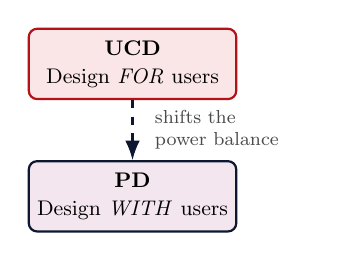
\begin{tikzpicture}[scale=0.85, transform shape]
        \node[pdboxRed, minimum width=3.1cm] (ucd) {\textbf{UCD}\\[1pt] Design \textit{FOR} users};
        \node[pdboxGreen, minimum width=3.1cm, below=0.9cm of ucd] (pd) {\textbf{PD}\\[1pt] Design \textit{WITH} users};
        \draw[pdarrow, dashed] (ucd) -- (pd);
        \node[right, align=left, font=\footnotesize, text=pdGrayText, text width=2.4cm]
          at ([xshift=6pt]$(ucd)!0.5!(pd)$) {shifts the\\power balance};
      \end{tikzpicture}
    \end{column}
  \end{columns}
\end{frame}
\begin{frame}{The Collaboration Model: How Knowledge Meets}
  \centering
  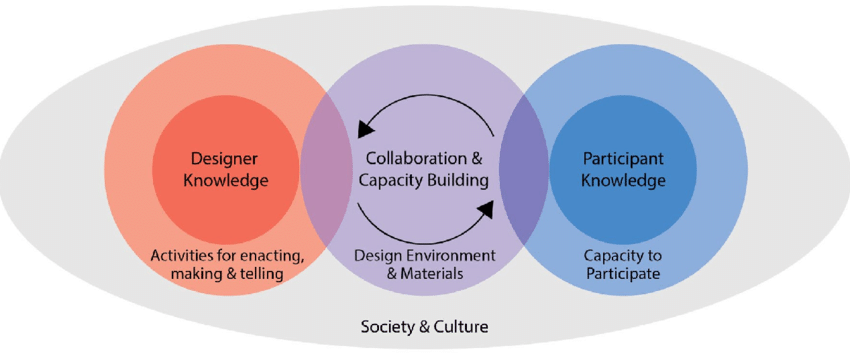
\includegraphics[width=0.86\textwidth]{collab_model.png}
  
  \pause
  \vspace{6pt}
  \begin{block}{\small In simple words}
    \footnotesize Designers bring \textbf{professional design knowledge};
    participants bring \textbf{lived, real-world knowledge}. Where the two
    overlap, real \textbf{collaboration and capacity-building} happens --
    supported by shared materials and a design environment, all inside a
    wider \textbf{society \& culture}.
  \end{block}
\end{frame}

\begin{frame}{Historical Context \& Evolution}
  \centering
  \null\vfill
  \vspace{18pt}
  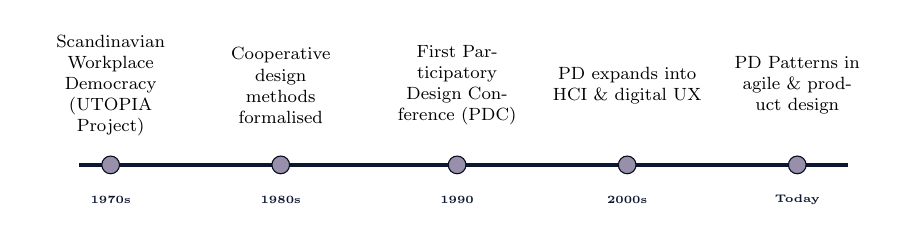
\begin{tikzpicture}[scale=0.8, transform shape]
    \draw[pdTeal, line width=1.6pt] (0,0) -- (12.2,0);
    \foreach \x/\lbl/\yr in {
        0.5/{Scandinavian\\Workplace Democracy\\(UTOPIA Project)}/{1970s},
        3.2/{Cooperative design\\methods formalised}/{1980s},
        6.0/{First Participatory\\Design Conference (PDC)}/{1990},
        8.7/{PD expands into\\HCI \& digital UX}/{2000s},
        11.4/{PD Patterns in\\agile \& product design}/{Today}
      }{
        \node[milestone] at (\x,0) {};
        \node[font=\footnotesize, align=center, text width=2.4cm, yshift=6pt] at (\x,1.05) {\lbl};
        \node[font=\bfseries\tiny, pdTeal] at (\x,-0.55) {\yr};
      }
  \end{tikzpicture}

  \vspace{14pt}
  \begin{alertblock}{\small Key milestone}
    \footnotesize The \textbf{UTOPIA Project (Scandinavia, late 1970s--80s)}
    united Nordic trade unions with researchers to let \textit{typesetters}
    co-design their own new computer tools -- the origin of PD.
  \end{alertblock}
  \vfill\null
\end{frame}

\begin{frame}{The Problem Before Participatory Design}
  \begin{columns}[T,onlytextwidth]
    \begin{column}{0.5\textwidth}
      \begin{alertblock}{Top-down, designer-centric era}
        \small Decisions flowed in \textbf{one direction only} -- from
        experts down to the people who actually used the system.
      \end{alertblock}
      \begin{itemize}
        \item<1-> Management \& designers decided \textbf{alone}
        \item<2-> Users' real needs, context, and expertise \textbf{ignored}
        \item<3-> Feedback arrived only \textbf{after} launch -- too late
      \end{itemize}
    \end{column}
    \begin{column}{0.46\textwidth}
      \centering
      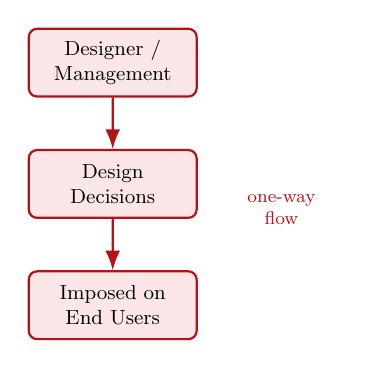
\begin{tikzpicture}[scale=0.82, transform shape, node distance=8mm]
        \node[pdboxRed] (a) {Designer /\\Management};
        \node[pdboxRed, below=of a] (b) {Design\\Decisions};
        \node[pdboxRed, below=of b] (c) {Imposed on\\End Users};
        \draw[pdarrow, pdRed] (a) -- (b);
        \draw[pdarrow, pdRed] (b) -- (c);
        \node[font=\footnotesize, align=center, text width=2cm, pdRed]
          at ([xshift=13mm, yshift=-4mm]b.east) {one-way\\flow};
      \end{tikzpicture}
    \end{column}
  \end{columns}
  \vspace{4pt}
  \begin{block}<4->{\small Result}
    \footnotesize Poor usability, low adoption, workplace resistance, and
    tools that solved the \textit{wrong} problem.
  \end{block}
\end{frame}


\begin{frame}{How Participatory Design Solved It}
  \centering
  \null\vfill
  \vspace{20pt}
  \begin{columns}[T,onlytextwidth]
    \begin{column}{0.47\textwidth}
      \centering
      {\small\bfseries\color{pdRed} Before: Top-Down}\\[6pt]
      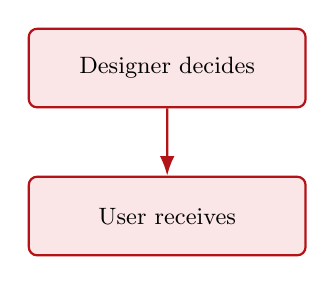
\begin{tikzpicture}[scale=0.95, transform shape, node distance=9mm]
        \node[pdboxRed, minimum width=3.7cm] (d1) {Designer decides};
        \node[pdboxRed, minimum width=3.7cm, below=of d1] (d2) {User receives};
        \draw[pdarrow, pdRed] (d1) -- (d2);
      \end{tikzpicture}
    \end{column}
    \begin{column}{0.47\textwidth}
      \centering
      {\small\bfseries\color{pdTeal!20} After: Participatory}\\[6pt]
      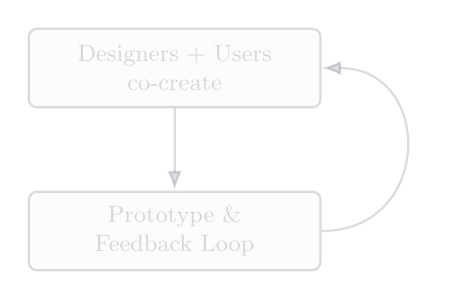
\begin{tikzpicture}[scale=0.95, transform shape, node distance=11mm]
        \begin{scope}[opacity=0.15]
        \node[pdboxGreen, minimum width=3.9cm] (p1) {Designers + Users\\co-create};
        \node[pdboxGreen, minimum width=3.9cm, below=of p1] (p2) {Prototype \&\\Feedback Loop};
        \draw[pdarrow, pdTeal] (p1) -- (p2);
        \draw[pdarrow, pdTeal] (p2.east) .. controls +(1.5,0) and +(1.5,0) .. (p1.east);
        \end{scope}
      \end{tikzpicture}
    \end{column}
  \end{columns}
  \vfill\null
\end{frame}

\begin{frame}{How Participatory Design Solved It}
  \centering
  \null\vfill
  \vspace{20pt}
  \begin{columns}[T,onlytextwidth]
    \begin{column}{0.47\textwidth}
      \centering
      {\small\bfseries\color{pdRed} Before: Top-Down}\\[6pt]
      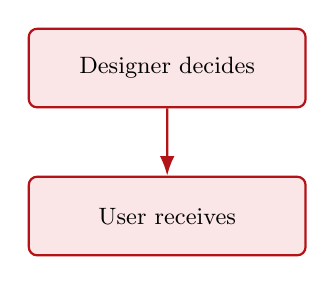
\begin{tikzpicture}[scale=0.95, transform shape, node distance=9mm]
        \node[pdboxRed, minimum width=3.7cm] (d1) {Designer decides};
        \node[pdboxRed, minimum width=3.7cm, below=of d1] (d2) {User receives};
        \draw[pdarrow, pdRed] (d1) -- (d2);
      \end{tikzpicture}
    \end{column}
    \begin{column}{0.47\textwidth}
      \centering
      {\small\bfseries\color{pdTeal} After: Participatory}\\[6pt]
      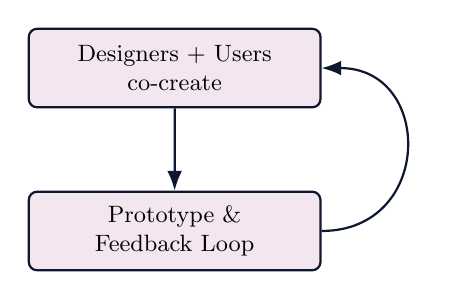
\begin{tikzpicture}[scale=0.95, transform shape, node distance=11mm]
        \node[pdboxGreen, minimum width=3.9cm] (p1) {Designers + Users\\co-create};
        \node[pdboxGreen, minimum width=3.9cm, below=of p1] (p2) {Prototype \&\\Feedback Loop};
        \draw[pdarrow, pdTeal] (p1) -- (p2);
        \draw[pdarrow, pdTeal] (p2.east) .. controls +(1.5,0) and +(1.5,0) .. (p1.east);
      \end{tikzpicture}
    \end{column}
  \end{columns}
  \vspace{10pt}
  \begin{exampleblock}{\small What changed}
    \footnotesize Empowerment replaced imposition: stakeholders gained a
    \textbf{real voice and decision power}, and design became an
    \textbf{iterative, cyclical conversation} rather than a one-time handoff.
  \end{exampleblock}
  \vfill\null
\end{frame}


\begin{frame}{Core Principles: Mutual Learning}
  \centering
  \null\vfill
  \begin{tikzpicture}[scale=1.0, transform shape]
    \node[pdbox, text width=10cm, minimum height=5.5cm, align=center]
      at (0,0) {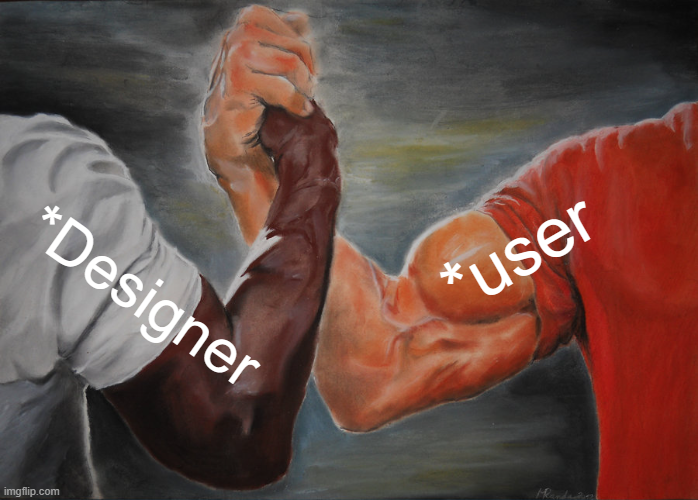
\includegraphics[width=5cm,height=2.5cm,keepaspectratio]{biceps.png}\\[10pt]
      {\Large\textbf{Mutual Learning}}\\[8pt]
      {\normalsize Designers learn the domain; users learn design thinking.\\[3pt]
      Knowledge flows both ways, building shared understanding.}};
  \end{tikzpicture}
  \vfill\null
\end{frame}
 
\begin{frame}{Core Principles: Co-creation \& Ownership}
  \centering
  \null\vfill
  \begin{tikzpicture}[scale=1.0, transform shape]
    \node[pdbox, text width=10cm, minimum height=5.5cm, align=center]
      at (0,0) {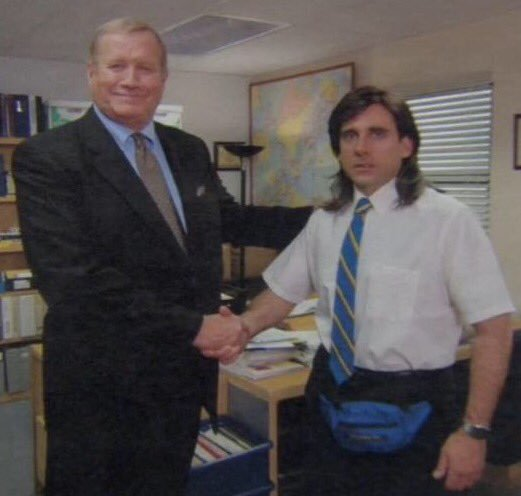
\includegraphics[width=5cm,height=2.5cm,keepaspectratio]{handshake.jpg}\\[10pt]
      {\Large\textbf{Co-creation \& Ownership}}\\[8pt]
      {\normalsize Build it together, so it feels like theirs.\\[3pt]
      Shared ownership leads to stronger buy-in and better outcomes.}};
  \end{tikzpicture}
  \vfill\null
\end{frame}


\begin{frame}{Core Principles: Iterative Prototyping}
  \centering
  \null\vfill
  \begin{tikzpicture}[scale=1.0, transform shape]
    \node[pdbox, text width=10cm, minimum height=5.5cm, align=center]
      at (0,0) {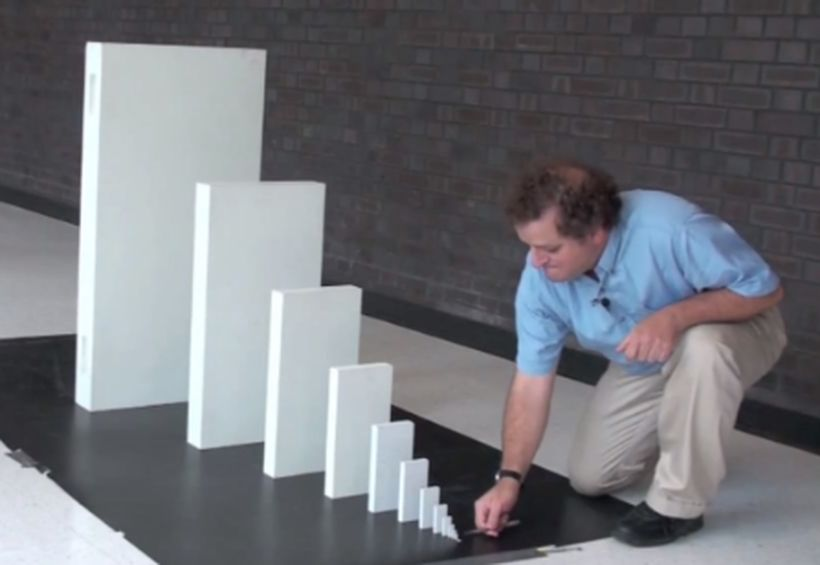
\includegraphics[width=5cm,height=2.5cm,keepaspectratio]{tiles.jpg}\\[10pt]
      {\Large\textbf{Iterative Prototyping}}\\[8pt]
      {\normalsize Small steps and testing, not one big launch.\\[3pt]
      Rapid cycles of build--test--refine keep design grounded in reality.}};
  \end{tikzpicture}
  \vfill\null
\end{frame}
\begin{frame}{Core Principles: Democratic Decision-Making}
  \centering
  \null\vfill
  \begin{tikzpicture}[scale=1.0, transform shape]
    \node[pdbox, text width=10cm, minimum height=5.5cm, align=center]
      at (0,0) {
\includegraphics[width=5cm,height=2.5cm,keepaspectratio]{rollsafe.jpg}\\[10pt]
      {\Large\textbf{Democratic Decision-Making}}\\[8pt]
      {\normalsize No single voice controls everything.\\[3pt]
      Every stakeholder has an equal seat at the table.}};
  \end{tikzpicture}
  \vfill\null
\end{frame}
\begin{frame}{Same Idea, Explained by a Cat}
  \centering
  \null\vfill
  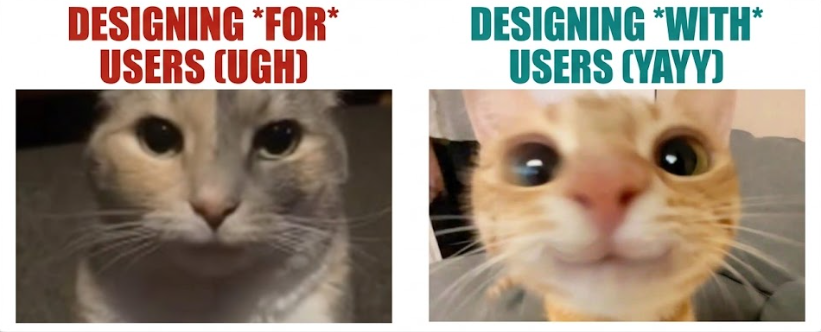
\includegraphics[width=0.78\textwidth]{cat_meme.png}\\[6pt]
  {\footnotesize\color{pdGrayText} Because sometimes a grumpy cat explains
  user research better than a slide ever could.}
  \vfill
  {\small\color{pdTeal}\textbf{Next:} Asef will cover processes and techniques of implementing Participatory Design Method.}
\end{frame}

\end{document}